% Mémo technique : fonctionnement de SeldonH
% Compilation : pdflatex memo_technique_SeldonH.tex (deux passes)
\documentclass[11pt,a4paper]{article}
\usepackage[T1]{fontenc}
\usepackage[utf8]{inputenc}
\usepackage{lmodern}
\IfFileExists{french.ldf}%
  {\usepackage[french]{babel}}%
  {\usepackage{babel}\babelprovide[import,main]{french}}
\providecommand{\og}{«~}\providecommand{\fg}{\unskip~»}
\usepackage[margin=2.2cm]{geometry}
\usepackage{xcolor}
\usepackage{booktabs,tabularx}
\usepackage{enumitem}
\usepackage{float}
\usepackage{caption}
\usepackage{amsmath,amssymb}
\usepackage{tikz}
\usetikzlibrary{arrows.meta,positioning,fit,backgrounds,calc,shapes.geometric}
\usepackage[hidelinks]{hyperref}

\definecolor{cmblue}{RGB}{40,90,160}
\definecolor{ui}{RGB}{225,236,250}
\definecolor{pre}{RGB}{255,243,214}
\definecolor{llm}{RGB}{232,224,248}
\definecolor{calc}{RGB}{220,242,224}
\definecolor{out}{RGB}{250,226,226}
\definecolor{store}{RGB}{236,236,236}

\newcommand{\code}[1]{\texttt{\small #1}}

% ---------- environnement d'algorithme (sans paquet externe) ----------
\newfloat{algorithme}{tbp}{loa}
\floatname{algorithme}{Algorithme}
\floatstyle{ruled}\restylefloat{algorithme}
\newcounter{algl}
\newlength{\algind}\setlength{\algind}{1.2em}
\newenvironment{algo}{%
  \begin{list}{\scriptsize\arabic{algl}}{\usecounter{algl}%
    \setlength{\itemsep}{0pt}\setlength{\parsep}{0pt}\setlength{\topsep}{2pt}%
    \setlength{\leftmargin}{2.2em}\setlength{\labelwidth}{1.6em}\small}}%
  {\end{list}}
\newcommand{\Li}[2]{\item\hspace*{#1\algind}#2}
\newcommand{\Kw}[1]{\textbf{#1}}
\newcommand{\Com}[1]{\hfill{\color{gray}\textit{\footnotesize #1}}}

\title{\textbf{SeldonH} --- Mémo technique\\[2pt]\large Fonctionnement général de l'application}
\author{Philippe Dufresne}
\date{4 novembre 2026}

\begin{document}
\maketitle

\begin{abstract}
SeldonH est une application Qt/C++ de dialogue avec un modèle de langage (local par llama.cpp, ou distant par une API
compatible OpenAI) destinée aux archéologues et géologues. Elle réalise des datations simples, calcule des Events au sens
de ChronoModel, produit des fichiers de modèle \code{.chr} et aide à interpréter les résultats. Le principe directeur est
de \emph{séparer le langage du calcul} : le modèle de langage comprend la question, choisit et commente ; tous les
calculs (calibrations, MCMC, fichiers) sont faits par du code C++ déterministe, porté de ChronoModel, sur l'ordinateur de
l'utilisateur. Ce mémo décrit l'architecture (graphe fonctionnel), l'algorithme général de traitement d'une question et
les principaux modules. Mise à jour du 4 novembre 2026 : mode calculatrice, calcul unique \code{relation} (termes de
provenances mélangées, corrélation, formules), tableaux de datations, serveur MCP, test automatique de l'appel d'outils, réglages CPU.
\end{abstract}

\tableofcontents

% =====================================================================
\section{Principes de conception}

\begin{enumerate}[leftmargin=*]
\item \textbf{Le modèle ne calcule jamais.} Un petit modèle ne sait pas calibrer et invente des règles. Les méthodes de
  datation sont donc reprises de ChronoModel en C++ (\code{src/methods/}) et exécutées localement. Le modèle reçoit le
  \emph{texte} des résultats exacts et les commente.
\item \textbf{Le modèle ne produit jamais le \code{.chr} complet.} Il écrit une spécification JSON courte (une dizaine
  de champs) ; \code{ChrBuilder} ajoute les quelque 200 champs obligatoires (identifiants, UUID, réglages MCMC, plage
  d'étude, positions\dots) et contrôle la cohérence.
\item \textbf{Connaissances par fiches.} Le savoir-faire est rangé dans des \emph{compétences} (fiches Markdown) choisies
  à chaque question selon ses mots-clés, dans un budget de texte. On enrichit l'application en ajoutant des fiches,
  sans recompiler.
\item \textbf{Un seul jeu de calculs pour trois transports.} Modèle local (bloc \code{```calcul}), modèle distant
  (appel d'outils natif) et autre assistant (serveur MCP \code{seldonh-mcp}) déclenchent les mêmes fonctions
  (\code{src/methods/common/Tools.*}) ; l'historique est identique, on peut changer de moteur en cours de conversation.
\item \textbf{La fiche de SeldonH est la seule source des chiffres.} Quand SeldonH a fait le calcul seul et que la
  question ne demande pas d'explication, le modèle n'est pas relancé (\emph{mode calculatrice}) ; sinon il reçoit les
  valeurs \og déjà affichées \fg{} avec la consigne de ne pas les recopier.
\item \textbf{Le modèle sélectionne, SeldonH manipule les valeurs.} Pour un tableau de datations, le modèle ne reçoit
  qu'un résumé et demande des sélections avec une action ; il ne recopie jamais une valeur.
\item \textbf{Confidentialité.} Avec le modèle local, rien ne quitte la machine. Avec un modèle distant, seuls la
  conversation, les fiches choisies, les pièces jointes et les paramètres d'appel d'outils sont envoyés ; les courbes
  de calibration et les calculs restent locaux. La clé API est rangée dans le trousseau du système (QtKeychain).
\end{enumerate}

% =====================================================================
\section{Graphe fonctionnel}

La figure~\ref{fig:graphe} montre les modules et les flux. Les flèches pleines sont les flux de données d'une question ;
les flèches en tirets sont les boucles (relance du modèle après un calcul, retour des résultats de ChronoModel).

\begin{figure}[p]
\centering
\resizebox{\textwidth}{!}{%
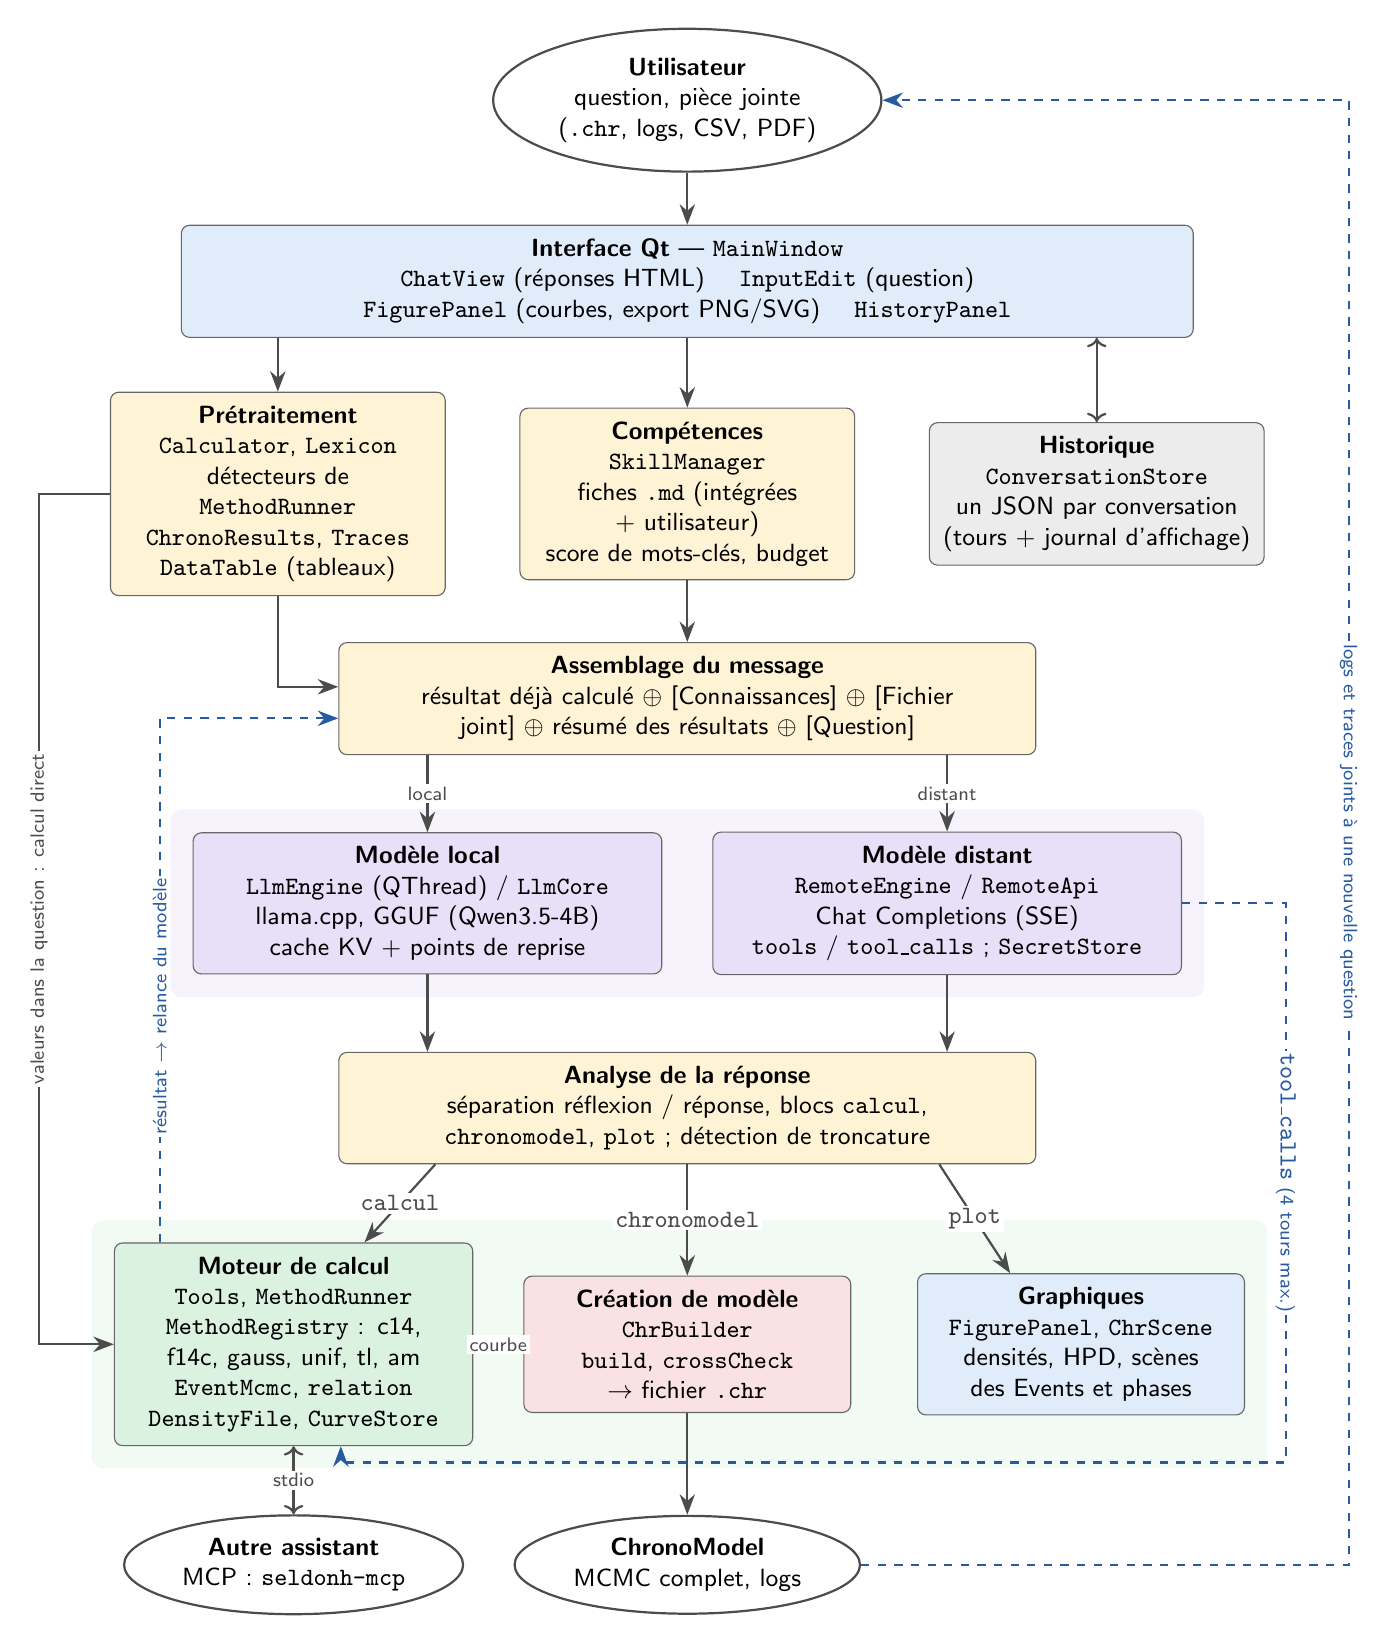
\begin{tikzpicture}[
  font=\sffamily\small,
  box/.style={draw=black!60, rounded corners=3pt, align=center, inner sep=5pt, minimum height=1.1cm, text width=#1},
  box/.default=3.6cm,
  ext/.style={draw=black!70, thick, ellipse, align=center, inner sep=3pt, fill=white},
  flow/.style={-{Stealth[length=2.6mm]}, thick, black!70},
  loop/.style={-{Stealth[length=2.6mm]}, thick, dashed, cmblue},
  lab/.style={font=\sffamily\scriptsize, fill=white, inner sep=1pt, align=center}
]
% --- utilisateur
\node[ext] (user) at (0,0) {\textbf{Utilisateur}\\ question, pièce jointe\\ (\code{.chr}, logs, CSV, PDF)};

% --- interface
\node[box=12.5cm, fill=ui] (ui) at (0,-2.3) {\textbf{Interface Qt} --- \code{MainWindow}\\
  \code{ChatView} (réponses HTML) \quad \code{InputEdit} (question) \quad \code{FigurePanel} (courbes, export PNG/SVG)
  \quad \code{HistoryPanel}};

% --- prétraitement
\node[box=3.9cm, fill=pre] (pre) at (-5.2,-5.0) {\textbf{Prétraitement}\\ \code{Calculator}, \code{Lexicon}\\
  détecteurs de \code{MethodRunner}\\ \code{ChronoResults}, \code{Traces}\\ \code{DataTable} (tableaux)};
\node[box=3.9cm, fill=pre] (skills) at (0,-5.0) {\textbf{Compétences}\\ \code{SkillManager}\\ fiches \code{.md}
  (intégrées + utilisateur)\\ score de mots-clés, budget};
\node[box=3.9cm, fill=store] (hist) at (5.2,-5.0) {\textbf{Historique}\\ \code{ConversationStore}\\ un JSON par
  conversation\\ (tours + journal d'affichage)};

% --- assemblage
\node[box=8.5cm, fill=pre] (prompt) at (0,-7.6) {\textbf{Assemblage du message}\\ résultat déjà calculé $\oplus$
  [Connaissances] $\oplus$ [Fichier joint] $\oplus$ résumé des résultats $\oplus$ [Question]};

% --- moteurs
\node[box=5.6cm, fill=llm] (local) at (-3.3,-10.2) {\textbf{Modèle local}\\ \code{LlmEngine} (QThread) /
  \code{LlmCore}\\ llama.cpp, GGUF (Qwen3.5-4B)\\ cache KV + points de reprise};
\node[box=5.6cm, fill=llm] (remote) at (3.3,-10.2) {\textbf{Modèle distant}\\ \code{RemoteEngine} / \code{RemoteApi}\\
  Chat Completions (SSE)\\ \code{tools} / \code{tool\_calls} ; \code{SecretStore}};

% --- analyse de la réponse
\node[box=8.5cm, fill=pre] (parse) at (0,-12.8) {\textbf{Analyse de la réponse}\\ séparation réflexion / réponse,
  blocs \code{calcul}, \code{chronomodel}, \code{plot} ; détection de troncature};

% --- sorties
\node[box=4.2cm, fill=calc] (calc) at (-5.0,-15.8) {\textbf{Moteur de calcul}\\ \code{Tools}, \code{MethodRunner}\\
  \code{MethodRegistry} : c14, f14c, gauss, unif, tl, am\\ \code{EventMcmc}, \code{relation}\\ \code{DensityFile},
  \code{CurveStore}};
\node[ext] (mcp) at (-5.0,-18.6) {\textbf{Autre assistant}\\ MCP : \code{seldonh-mcp}};
\node[box=3.8cm, fill=out] (chr) at (0,-15.8) {\textbf{Création de modèle}\\ \code{ChrBuilder}\\ \code{build},
  \code{crossCheck}\\ $\rightarrow$ fichier \code{.chr}};
\node[box=3.8cm, fill=ui] (fig) at (5.0,-15.8) {\textbf{Graphiques}\\ \code{FigurePanel}, \code{ChrScene}\\
  densités, HPD, scènes\\ des Events et phases};

\node[ext] (cm) at (0,-18.6) {\textbf{ChronoModel}\\ MCMC complet, logs};

% --- flux
\draw[flow] (user) -- (ui);
\draw[flow] (ui.south -| pre.north) -- (pre.north);
\draw[flow] (ui.south) -- (skills.north);
\draw[flow, <->] (ui.south -| hist.north) -- (hist.north);
\draw[flow] (pre.south) |- ($(prompt.west)+(0,0.15)$);
\draw[flow] (skills) -- (prompt);
\draw[flow] (prompt.south -| local.north) -- node[lab]{local} (local.north);
\draw[flow] (prompt.south -| remote.north) -- node[lab]{distant} (remote.north);
\draw[flow] (local.south) -- (local.south |- parse.north);
\draw[flow] (remote.south) -- (remote.south |- parse.north);
\draw[flow] (parse.south -| chr.north) -- node[lab]{\code{chronomodel}} (chr.north);
\draw[flow] ($(parse.south)+(-3.2,0)$) -- node[lab]{\code{calcul}} ($(calc.north)+(0.9,0)$);
\draw[flow] ($(parse.south)+(3.2,0)$) -- node[lab]{\code{plot}} ($(fig.north)+(-0.9,0)$);
\draw[flow] (calc.east) -- node[lab]{courbe} (calc.east -| chr.west) ;
\draw[flow] (chr) -- (cm);
\draw[flow, <->] (mcp) -- node[lab]{stdio} (calc);

% calcul direct depuis la question (sans le modèle)
\draw[flow] (pre.west) -- ++(-0.9,0) |- node[lab, pos=0.25, rotate=90]{valeurs dans la question : calcul direct} (calc.west);

% appel d'outils natif (distant)
\draw[loop] (remote.east) -- (7.6,0 |- remote.east) -- node[lab, rotate=-90]{\code{tool\_calls} (4 tours max.)} (7.6,-17.3) -| ($(calc.south)+(0.6,0)$);
% relance avec le résultat
\draw[loop] ($(calc.north)+(-1.7,0)$) -- node[lab, rotate=90, pos=0.45]{résultat $\rightarrow$ relance du modèle} ($(calc.north |- prompt.west)+(-1.7,-0.25)$) -- ($(prompt.west)+(0,-0.25)$);
% retour des logs
\draw[loop] (cm.east) -- (8.4,0 |- cm.east) |- node[lab, pos=0.25, rotate=-90]{logs et traces joints à une nouvelle question} (user.east);


% légende des groupes
\begin{scope}[on background layer]
  \node[fill=llm!40, rounded corners, fit=(local)(remote), inner sep=8pt] {};
  \node[fill=calc!40, rounded corners, fit=(calc)(chr)(fig), inner sep=8pt] {};
\end{scope}
\end{tikzpicture}}
\caption{Graphe fonctionnel de SeldonH. La réponse est affichée en flux dans l'interface pendant sa génération. Orange : préparation et analyse du texte ; violet : moteurs de langage ;
vert : calculs locaux déterministes ; rouge : création du modèle ChronoModel ; gris : stockage.}
\label{fig:graphe}
\end{figure}

\subsection*{Rôle des modules}
\begin{center}\small
\begin{tabularx}{\textwidth}{@{}l X@{}}
\toprule
\textbf{Module} & \textbf{Rôle} \\ \midrule
\code{MainWindow} & Orchestration d'une question (algorithme~\ref{alg:general}), gestion des tours, mode
  calculatrice, liens \code{seldon://} (enregistrer un \code{.chr}, un fichier de densité, un extrait de tableau,
  demander un commentaire, déplier le raisonnement, rappeler une figure). \\
\code{ChatView}, \code{MathText} & Rendu Markdown $\rightarrow$ HTML, formules LaTeX du modèle $\rightarrow$ HTML. \\
\code{FigurePanel}, \code{ChrScene} & Courbes (densités, HPD remplie, superposition ou une densité par ligne), nuages de points (corrélation), export
  PNG/SVG, scènes des Events et des phases d'un \code{.chr}. \\
\code{Calculator} & Calculatrice locale (\og 2+3 \fg, \code{ADtoBP(-550)}) sans appel au modèle. \\
\code{Lexicon} & Ramène une question en espagnol, italien ou allemand aux mots-clés français. \\
\code{SkillManager} & Lecture des fiches (en-tête : \code{keywords}, \code{priority}, \code{always}) et sélection. \\
\code{LlmCore} / \code{LlmEngine} & Enveloppe C++ de llama.cpp (sans Qt) ; adaptateur Qt dans un \code{QThread}. \\
\code{RemoteEngine} / \code{RemoteApi} & API Chat Completions compatible OpenAI, flux SSE, appel d'outils. \\
\code{ToolsProbe} & Test automatique de l'appel d'outils d'un serveur distant (natif, en texte, ignoré, refusé),
  mémorisé par serveur et modèle pendant 30 jours. \\
\code{CpuTopology} & Nombre de threads \og automatique \fg{} : cœurs physiques performance (génération) et tous les
  cœurs physiques (prompt), sous macOS, Linux et Windows. \\
\code{AutoTune} & \og Optimiser pour ce modèle \fg{} : contexte, longueur de réponse, budget des fiches. \\
\code{MethodRunner}, \code{Tools} & Détecteurs de datations et de relations, normalisation et validation des
  requêtes, exécution (dont \code{relation}, §\ref{sec:relation}), fiche de résultat, texte pour le modèle ; définition
  des 14 outils. \\
\code{MethodRegistry} & Une classe \code{Method} par technique (c14, f14c, gauss, unif, tl, am). \\
\code{EventMcmc} & Estimation bayésienne d'un Event (modèle EDM2), diagnostics $\hat R$ et ESS. \\
\code{CurveStore}, \code{RefCurve} & Courbes de référence : dossier utilisateur, \code{Calib} de ChronoModel, courbes
  intégrées. \\
\code{ChrBuilder} & Spécification JSON $\rightarrow$ \code{.chr} valide ; contraintes en toutes lettres ;
  vérification croisée avec le texte de l'utilisateur. \\
\code{ChronoResults} & Lecture des logs et résultats de ChronoModel joints, résumé dans un budget. \\
\code{Traces} & Chaînes MCMC exportées par ChronoModel (\code{Chain\_all\_Events.csv}, \code{Chain\_all\_Phases.csv}\dots),
  gardées tirage par tirage ; noms de colonnes en clair (\og début de la phase A \fg{} $\rightarrow$
  \code{Phase A Begin}). \\
\code{DataTable}, \code{Spreadsheet} & Tableaux de datations (\code{.xlsx}, \code{.ods}, CSV, collés) : rôles des
  colonnes, méthode de chaque ligne, sélections, actions (§\ref{sec:tableaux}). \\
\code{McpServer} & Serveur MCP \code{seldonh-mcp} (QtCore seul) : les 14 outils pour un autre assistant. \\
\code{ConversationStore} & Historique (écriture atomique \code{QSaveFile}). \\
\bottomrule
\end{tabularx}
\end{center}

% =====================================================================
\section{Algorithme général}

L'algorithme~\ref{alg:general} décrit le traitement d'une question, de la saisie à l'enregistrement de la conversation.
Les étapes 1 à 4 sont des \emph{courts-circuits} : elles répondent sans le modèle de langage.

\begin{algorithme}[tbp]
\caption{Traitement d'une question (\code{MainWindow::sendMessage} et suite)}\label{alg:general}
\textbf{Entrées :} question $q$, pièce jointe éventuelle $a$, conversation $C$ (tours précédents), réglages
(format de date, budget $B$ des fiches, moteur).\\
\textbf{Sorties :} réponse affichée, figures, éventuel fichier \code{.chr}, conversation enregistrée.
\begin{algo}
\Li0{\Kw{si} $q$ = \code{/aide} \Kw{alors} afficher le mode d'emploi ; \Kw{fin}}
\Li0{\Kw{si} \code{Calculator.isCalculation}$(q)$ \Kw{alors} afficher le résultat exact ; \Kw{fin}
  \Com{rien n'est envoyé au modèle}}
\Li0{\Kw{si} $q$ demande un dessin \Kw{et} un \code{.chr} est connu \Kw{alors} dessiner les scènes ;}
\Li1{\Kw{si} la question ne demande que le dessin \Kw{alors} \Kw{fin}}
\Li0{\Kw{si} $q$ ou $a$ contient un tableau de datations \Kw{alors} le lire comme tableau courant, afficher sa fiche ;}
\Li1{\Kw{si} il n'y a pas d'autre consigne \Kw{alors} \Kw{fin}}
\Li0{$D \leftarrow$ \code{recentDatings}$(C)$ \Com{datations des 8 dernières questions}}
\Li0{\Kw{si} \code{requestsFromQuestion}$(q) \ne \emptyset$ \Kw{ou} \code{relationWithPrevious}$(q, D) \ne \emptyset$}
\Li1{\Kw{et} \code{asksCommentary}$(q)$ est faux \Kw{alors} calculer, afficher la fiche et le lien
  \og Demander un commentaire \fg ; \Kw{fin}}
\Li1{\Com{mode calculatrice : aucune génération, marche sans modèle chargé}}
\Li0{\Kw{si} aucun modèle de langage n'est prêt \Kw{alors} message d'état ; \Kw{fin}}
\Li0{$q_k \leftarrow$ \code{Lexicon.translate}$(q)$ \Com{mots-clés en français}}
\Li0{$m \leftarrow$ \code{isModelRequest}$(q_k)$ ; \quad $M \leftarrow$ \code{datingMethodsIn}$(q_k)$}
\Li0{$P \leftarrow$ fiches imposées : 03 si $m$ ; 13 si âge-profondeur ; fiche de chaque méthode de $M$ ;}
\Li1{19 (phases, Events) ou 11 (logs) si des résultats ChronoModel sont présents ; 21 si une relation est demandée ;}
\Li1{22 et résumé du tableau courant s'il y en a un}
\Li0{$K \leftarrow$ \code{SkillManager.select}$(q_k,\ m\ ?\ 0 : B,\ \text{exclues},\ P)$ \Com{voir §\ref{sec:skills}}}
\Li0{$R \leftarrow$ \code{MethodRunner.analyzeQuestion}$(q)$ \Com{valeurs écrites dans la question}}
\Li0{\Kw{si non} $R$.trouvé \Kw{alors} $R \leftarrow$ recalcul de la datation précédente (autre niveau, autre période)}
\Li0{\Kw{si} $R$.trouvé \Kw{alors} afficher la fiche (HPD, médiane, mode) et la densité}
\Li0{$u \leftarrow R.\text{texte} \oplus K \oplus a \oplus \text{résumé des résultats} \oplus q$
  \Com{message vu par le modèle}}
\Li0{ajouter le tour $(q, u)$ à $C$ ; enregistrer $C$}
\Li0{\Kw{répéter} \Com{boucle agent}}
\Li1{générer la réponse en flux (local : gabarit + cache KV ; distant : SSE avec déclaration des outils)}
\Li1{\Kw{tant que} le moteur distant renvoie des \code{tool\_calls} \Kw{et} tours $\le 4$ \Kw{faire}}
\Li2{exécuter chaque outil localement (\code{Tools}) ; réinjecter le texte du résultat ; poursuivre}
\Li1{afficher la réponse : réflexion séparée, blocs \code{calcul}/\code{chronomodel} masqués, \code{plot} $\rightarrow$
  panneau}
\Li1{\Kw{si} bloc \code{chronomodel} \Kw{alors}}
\Li2{$S \leftarrow$ spécification ; \code{ChrBuilder.build}$(S)$ ; \code{crossCheck}$(S, q)$}
\Li2{afficher le résumé, les avertissements et le lien \og Enregistrer le modèle (\code{.chr}) \fg}
\Li1{\Kw{si} bloc \code{calcul} \Kw{et} le tour n'a pas déjà été calculé \Kw{alors}}
\Li2{$R' \leftarrow$ \code{MethodRunner.run}(blocs) ; afficher fiche et figures}
\Li2{\Kw{si} la question ne demande pas d'explication \Kw{alors} sortir \Com{mode calculatrice}}
\Li2{ajouter un tour synthétique $u \leftarrow R'.\text{texte}$ ; \Kw{continuer} \Com{le modèle commente}}
\Li1{\Kw{sinon} sortir de la boucle}
\Li0{\Kw{si} la réponse est coupée (limite de longueur, contexte plein, flux interrompu) \Kw{alors}}
\Li1{proposer \og Continuer la réponse \fg{} (la suite s'ajoute au même tour)}
\Li0{enregistrer $C$ (tours + journal d'affichage)}
\end{algo}
\end{algorithme}

\paragraph{Remarques.}
\begin{itemize}[leftmargin=*]
\item Un calcul est fait \emph{au plus une fois} par question : un tour marqué \og déjà calculé \fg{} (\code{followUp})
  ne relance pas de calcul, ce qui évite les boucles avec le modèle local.
\item Le modèle local n'a qu'un tour de suite après un bloc \code{calcul} ; le modèle distant peut enchaîner jusqu'à
  4 appels d'outils, puis la requête est envoyée avec \code{tool\_choice: none}.
\item Si le serveur distant refuse le champ \code{tools}, la requête est rejouée sans outils et le bloc \code{calcul}
  prend le relais. Un appel d'outil est réécrit en bloc \code{calcul} dans l'historique.
\item Les fiches des tours passés ne sont pas renvoyées : seul le tour courant les reçoit, ce qui garde le prompt court.
\item Un tour en mode calculatrice (\code{calcOnly}) n'a pas de réponse du modèle : il n'est pas envoyé comme paire
  question / réponse, mais placé en contexte en tête du message suivant (\code{calcOnlyContext}), faute de quoi un petit
  modèle recopiait le texte de remplacement. L'export du prompt montre exactement ce qui est envoyé.
\item Préférence \og Commentaire après un calcul \fg{} : si la question le demande (défaut), jamais, toujours.
\end{itemize}

% =====================================================================
\section{Sélection des compétences}\label{sec:skills}

Chaque fiche \code{.md} porte un en-tête (\code{name}, \code{description}, \code{keywords}, \code{priority},
\code{always}). La fiche d'identité (\code{always: true}) va dans le message système ; les autres sont placées devant
la question. Le score d'une fiche pour une question $q$ (sans accents, en minuscules) est
\[
  s = 10\Big(\sum_{k \in \text{mots-clés}} w(k) + \sum_{w \in \text{description}} [\,w \in q\,]\Big) + \text{priorité},
\]
\[
  w(k) = \begin{cases} 4 & k \text{ expression trouvée dans } q\\ 3 & k \text{ mot de } q \\
  2 & |k|>4 \text{ et } k \text{ sous-chaîne de } q \text{ (pluriel, préfixe),}\\ 0 & \text{sinon.}\end{cases}
\]
Les fiches imposées passent d'abord, puis les fiches par score décroissant tant que le budget (6000 caractères par
défaut) n'est pas dépassé. Pour une création de modèle, le budget est mis à zéro : seules la fiche commune (03) et
les fiches des méthodes citées sont fournies (exemple réel : 6\,100 caractères au lieu de 18\,500). Une fiche
utilisateur de même nom remplace la fiche intégrée.

% =====================================================================
\section{Moteurs de langage}

\subsection{Modèle local (llama.cpp)}
\code{LlmCore} formate la conversation avec le gabarit du modèle, n'évalue que le texte nouveau (cache KV), génère
en flux et oublie les plus anciens échanges si le contexte est plein. Modèle recommandé : Qwen3.5-4B en
Q4\_K\_M ($\approx 2{,}7$~Go, Apache~2.0), réflexion désactivée par défaut (préfixe \code{<think></think>} vide) ; le
bouton \og Réfléchir \fg{} l'active, grisé si le gabarit n'a pas \code{enable\_thinking}. Le raisonnement peut être
affiché (replié sous la réponse) mais n'est jamais renvoyé au modèle.

\paragraph{Performances CPU.} llama.cpp b11794. Sur macOS, une compilation par architecture puis \code{lipo} : le
build universel en un seul passage tombait en \code{GGML\_CPU\_GENERIC} (ni NEON optimisé, ni AVX2) ; gain mesuré
$\times 2{,}2$ (6,8 $\rightarrow$ 15,7~tok/s, i9-8950HK, Qwen3.5-2B). Threads \og automatique \fg{} : cœurs physiques
performance pour la génération, tous les cœurs physiques pour le prompt (\code{CpuTopology}) ; au-delà des cœurs libres
le débit s'effondre (attente active de ggml) quand un MCMC ou l'interface tourne en même temps.

\paragraph{Modèles hybrides.} Qwen3.5 mêle couches récurrentes (Gated DeltaNet) et couches d'attention ; l'état
récurrent ne peut pas être raccourci. \code{LlmCore} sauve donc au plus trois \emph{points de reprise} de l'état récurrent
($\approx 50$~Mo chacun) : fin du message système, début et fin du dernier message utilisateur. Au tour suivant, on
restaure le point le plus avancé contenu dans le préfixe commun, puis on raccourcit les couches d'attention.

\subsection{Modèle distant}
\code{RemoteEngine} parle à toute API Chat Completions compatible OpenAI (Base URL + clé). Réponse en flux SSE ;
troncature détectée par \code{finish\_reason: "length"} ou par l'absence de \code{[DONE]}. Les 14 outils
(\code{calibrer\_radiocarbone}, \code{calibrer\_f14c}, \code{dater\_luminescence}, \code{densite\_gauss},
\code{densite\_uniforme}, \code{dater\_archeomagnetisme}, \code{calculer\_evenement}, \code{combiner\_dates},
\code{comparer\_dates}, \code{analyser\_traces}, \code{calibration\_inverse}, \code{creer\_densite},
\code{courbes\_disponibles}, \code{tableau}) sont déclarés avec leur schéma ; leurs arguments sont validés et normalisés
(virgule décimale, nombres écrits en texte) et une valeur manquante renvoie une consigne au modèle sans lancer de calcul.
En mode calculatrice, les résultats ne sont pas renvoyés au serveur (sauf si un outil n'a pas pu s'exécuter).

\paragraph{Appel d'outils : Automatique / Toujours / Jamais.} En automatique, \code{ToolsProbe} envoie une requête
factice (outil \code{verifier\_outil}, température~0) et classe la réponse : natif (\code{tool\_calls}), appel écrit
dans le texte, ignoré, refusé, ou inconnu (réseau, 401, 429 : rien n'est conclu). Le résultat est mémorisé par serveur
et modèle pendant 30~jours ; un refus vu en conversation aussi.

% =====================================================================
\section{Calculs de datation}

\subsection{Dates isolées}
Chaque méthode (\code{src/methods/<id>/}) reprend la vraisemblance du plugin ChronoModel correspondant ; la densité est
calculée sur la grille de la courbe de référence avec un a priori uniforme, normalisée par la méthode des trapèzes,
tronquée à $10^{-5}$ ; les régions HPD (95~\% et 68~\% par défaut) sont obtenues par dichotomie sur le seuil de
densité. La fiche affiche HPD, médiane, mode, et la densité est tracée dans le panneau de droite. Les décimales affichées
suivent l'écart-type (deux chiffres significatifs) ou un réglage fixe.

\subsection{Calcul d'un Event (MCMC)}
\code{EventMcmc} porte le moteur de ChronoModel~4.0 pour un Event sans contrainte, modèle EDM2 :
\[
  y_i = t_i + \delta_i, \qquad t_i \sim \mathcal N(\theta, \sigma_i^2), \qquad
  \theta \sim \mathcal U[t_{\min}, t_{\max}], \qquad \sigma_i^2 \mid S_0^2 \sim \text{shrinkage}(S_0^2),
  \qquad S_0^2 \sim \text{Inv-Gamma}(1,\beta).
\]

\begin{algorithme}[htbp]
\caption{Échantillonnage d'un Event (\code{EventMcmc}, d'après \code{MCMCLoopChrono})}\label{alg:mcmc}
\begin{algo}
\Li0{\Kw{pour} chaque chaîne $c = 1..N_c$ (fil d'exécution séparé, graine propre) \Kw{faire}}
\Li1{initialiser $t_i$, $\sigma_i$, $\theta$ (\code{initialize\_time})}
\Li1{\Kw{chauffe} : \code{num\_burn} itérations}
\Li1{\Kw{adaptation} : par lots, jusqu'à ce que tous les taux d'acceptation soient dans leur fenêtre}
\Li2{(42--46~\% ; 30--40~\% pour $t_i$, $\sigma_i$ d'un Event à plusieurs dates), Robbins--Monro}
\Li1{\Kw{acquisition} : \code{num\_iter} itérations, éclaircissement \code{thinning}}
\Li2{\Kw{pour} chaque date $i$ : bloc $(t_i, \sigma_i, \delta_i)$ par Metropolis--Hastings
  (calibration + shrinkage)}
\Li2{décalage rigide $\theta + t_i$ ; Gibbs de $\theta$ : $\mathcal N(\mu, 1/P)$ tronquée à la période d'étude}
\Li2{marche adaptative sur $\log_{10} S_0^2$ ; recuit périodique ($T = 2^e$, $e$ décroissant)}
\Li0{densités a posteriori de $\theta$, $t_i$ : noyau gaussien, largeur de bande de Sheather--Jones}
\Li0{diagnostics : split-$\hat R$ rang-normalisé (bulk et tail), ESS bulk et tail}
\Li0{verdict : \og non convergé \fg{} si $\hat R \ge 1{,}05$ ou ESS $< 100 N_c$ ; \og satisfaisant \fg{} si
  $\hat R < 1{,}01$ et ESS $\ge 500 N_c$}
\end{algo}
\end{algorithme}

\subsection{Relations entre dates : un seul calcul \code{relation}}\label{sec:relation}
Une seule demande,
\begin{center}\code{\{"method":"relation", "op":…, "from":A, "to":B, "of":C\}}\end{center}
(outils \code{comparer\_dates} et \code{analyser\_traces}), avec six opérations : \code{value} (densité de $C$), \code{duration} ($B-A$ et
$P(B \text{ postérieur à } A)$), \code{between} (date uniforme entre $A$ et $B$), \code{order} ($P(A<B)$ et écart),
\code{inside} ($P(C \in [A ; B])$, avant, après) et \code{correlation} (matrice de corrélation et nuages de points de 2 à
8 termes, liste \code{terms}). Chaque terme peut être :
\begin{itemize}[leftmargin=*]
\item une \textbf{datation indépendante} : c14, f14c, tl, gauss, unif, am, \code{density} (fichier du plugin Density,
  lu dans \code{<racine>/Density}), \code{combine} ou \code{event} calculés par SeldonH, avec wiggle et période d'étude ;
  une datation écrite en texte (\og 2450 ± 30 BP \fg, \og TL 1700 ± 50 mesurée en 2025 \fg) est relue comme datation ;
\item une \textbf{colonne des traces chargées}, éventuellement prise dans plusieurs exports du \emph{même} calcul,
  par exemple \code{Chain\_all\_Events.csv} et \code{Chain\_all\_Phases.csv} (même nombre de tirages et mêmes
  chaînes, sinon refus) ;
\item une \textbf{année fixe} (\og -500 \fg, \og 500 av. J.-C. \fg).
\end{itemize}
\textbf{Calcul exact} quand il n'y a aucune colonne (sauf \code{between} et \code{correlation}) ; \textbf{tirage par
tirage} dès qu'il y a une colonne. Les colonnes sont prises telles quelles : la dépendance due aux contraintes et aux
phases est gardée, y compris entre deux fichiers d'export. Un mélange datation $+$ traces porte un avertissement : la
datation est supposée indépendante du modèle ChronoModel (sinon elle compte deux fois) et un Event de SeldonH n'a ni
contraintes ni phases.

\paragraph{Formules par opération.} Notations : $f_X$ et $F_X$ densité et fonction de répartition d'une datation
indépendante (grille régulière, intégrales par trapèzes) ; $a_i, b_i, c_i$ ($i=1..n$) valeurs du tirage $i$ (colonne de
traces, datation tirée ou année répétée) ; $\mathbf 1[\cdot]$ indicatrice ; $y$ année fixe.
\begin{center}\small
\renewcommand{\arraystretch}{1.35}
\begin{tabularx}{\textwidth}{@{}p{2.1cm} X X@{}}
\toprule
\textbf{Opération} & \textbf{Calcul exact (datations indépendantes)} & \textbf{Tirage par tirage (traces)} \\ \midrule
\code{order} &
  $D=B-A$, $f_D(d)=\int f_A(a)\,f_B(a+d)\,da$ (grille au plus petit pas) ; $P(A<B)=1-F_D(0)$. Année fixe :
  $f_D(d)=f_B(y+d)$ ou $f_A(y-d)$. &
  $P(A<B)=\frac1n\sum_i \mathbf 1[a_i<b_i]$ ; ex aequo comptés à part. \\
\code{duration} &
  densité $f_D$ ci-contre : HPD, mode, moyenne, quartiles ; $P(B>A)=1-F_D(0)$. &
  $d_i=b_i-a_i$, densité de $d$ par noyau ; $P(B>A)=\frac1n\sum_i\mathbf 1[b_i>a_i]$. \\
\code{between} &
  \multicolumn{2}{p{\dimexpr\textwidth-2.1cm-4\tabcolsep\relax}}{toujours par tirages ($10^5$ sans traces) :
  $t=\min(a_i,b_i)+U\,|b_i-a_i|$, $U\sim\mathcal U[0;1]$, 1 à 10 valeurs par tirage ; densité de $t$ par noyau.} \\
\code{inside} &
  $P(C\in[A;B])=\int f_C\,[F_A(1-F_B)+F_B(1-F_A)]\,dc$ ; $P(\text{avant})=\int f_C(1-F_A)(1-F_B)\,dc$ ;
  $P(\text{après})=\int f_C\,F_AF_B\,dc$ ; borne fixe : $F(c)=\mathbf 1[c\ge y]$. &
  $l_i=\min(a_i,b_i)$, $h_i=\max(a_i,b_i)$ ; $P(\text{dans})=\frac1n\sum_i\mathbf 1[l_i\le c_i\le h_i]$, avant :
  $c_i<l_i$, après : $c_i>h_i$. \\
\code{value} & $f_C$ elle-même. & densité des $c_i$ par noyau. \\
\code{correlation} &
  \multicolumn{2}{p{\dimexpr\textwidth-2.1cm-4\tabcolsep\relax}}{toujours par tirages communs ($10^5$ sans traces). Pearson
  $r=\sum_i(x_i-\bar x)(y_i-\bar y)\big/\sqrt{\sum_i(x_i-\bar x)^2\,\sum_i(y_i-\bar y)^2}$ ; Spearman $\rho$ = $r$ des
  rangs (rang moyen des ex aequo) ; intervalle approché à 95~\% : $\tanh\!\big(\operatorname{atanh} r\pm
  1{,}96/\sqrt{n_{\text{eff}}-3}\big)$, $n_{\text{eff}}$ = plus petit ESS bulk des deux colonnes ($n$ pour une datation
  tirée).} \\
\bottomrule
\end{tabularx}
\end{center}
\textbf{Datation tirée} : $t_k=F^{-1}\big((k+U_k)/n\big)$, $k=0..n-1$ (strates affectées dans un ordre aléatoire, graine
fixe 12345) : indépendante des colonnes par construction, donc de corrélation nulle avec elles. \textbf{Lissage} :
noyau gaussien, largeur de Sheather--Jones (Silverman en repli) ; HPD au niveau $p$ = $\{t : f(t)\ge s\}$ de masse $p$
($s$ par dichotomie). \textbf{Précision} : erreur Monte-Carlo d'une probabilité $\sqrt{p(1-p)/\text{ESS}}$ (ESS de
l'indicatrice sur les chaînes) ; $\hat R$ et ESS bulk / tail de la quantité calculée (durée, densité d'une colonne).

\paragraph{Corrélation (04/11/2026).} La fiche donne la matrice ($r$ au-dessus de la diagonale avec son intervalle,
$\rho$ au-dessous) ; l'op \code{correlation} ajoute un nuage de points par paire (3 au plus, 2\,500 tirages au plus,
droite $B=A$ en tirets ; axes inversés en format d'âge), tracé par \code{FigurePanel} (séries \code{"points"} et
\code{"dash"}, \code{"yreverse"}). Les autres opérations tirage par tirage ajoutent la matrice sans graphique. Détection
dans la question : \og corrélation \fg, \og covariance \fg, \og nuage de points \fg, \og varient ensemble \fg. Test
(\code{relationMixedSources}) : $r(\text{Four}, \text{Begin}) = 0{,}89$ (théorique $20/\sqrt{500}=0{,}894$),
$r(\text{Begin}, \text{End}) = 0{,}80$, $r(\text{Four}, \text{End}) = 0{,}71$ ($0{,}716$), $r \approx 0$ avec une
datation TL indépendante.

\paragraph{Vérification du 4 novembre 2026} (test \code{relationMixedSources}, deux exports synthétiques d'un même
calcul). Date TL $\rightarrow$ début de phase : durée $\mathcal N(-25 ; 54)$, $P = 32$~\% attendu et obtenu ; trace
d'un Event $\rightarrow$ fin de phase lue dans l'autre fichier : écart-type 18 (33,5 si les colonnes étaient
supposées indépendantes) ; TL, 14C, F14C, AM, uniforme, combinaison, Event de SeldonH et densité tabulée face à des
traces ; outils, questions directes et refus d'exports différents. Corrections faites à cette occasion : la datation
\code{density} n'était pas calculable (annoncée par les fiches et les outils) ; une datation sans nom mêlée à des
traces s'appelait \og A \fg, \og B \fg{} ou \og C \fg{} (confusion avec \og Phase A \fg) et porte maintenant le nom de
sa mesure (\og 14C 1650 ± 30 BP \fg) ; l'en-tête de la fiche nomme tous les fichiers de traces utilisés.

\paragraph{Datations des questions précédentes.} \og Combien de temps sépare la date précédente de\dots \fg{} :
\code{relationWithPrevious} reprend la ou les dernières datations de la conversation (il faut un renvoi et une
relation reconnue) ; pour une durée, la plus ancienne passe en premier.

\subsection{Tableaux de datations}\label{sec:tableaux}
\code{DataTable} lit un tableau (\code{.xlsx} et \code{.ods} par \code{QZipReader} + XML, CSV, TSV, Markdown ou
texte collé), cherche l'en-tête, reconnaît les rôles des colonnes en français et en anglais et déduit la méthode de
chaque ligne. Le tableau devient le \og tableau courant \fg{} de la conversation ; le modèle n'en reçoit qu'un résumé
et demande \code{\{"method":"table",…\}} avec une sélection (méthodes, lignes, noms, conditions \code{where}) et une
action : \code{extract} (CSV), \code{date} (récapitulatif), \code{event}, \code{combine}, \code{model} (\code{.chr} par
ligne ou par \code{group\_by}). Une erreur du modèle ne peut donc donner qu'une mauvaise sélection, visible dans la
fiche, jamais une mauvaise valeur.

\subsection{Autres calculs}
\begin{itemize}[leftmargin=*]
\item \code{DensityFile} : fichier de densité pour le plugin Density de ChronoModel (lois normale, log-normale,
  uniforme, triangulaire, trapézoïdale, exponentielle, gamma, bêta ; placement $t = \text{offset} \pm x$).
\item \code{Combination}, \code{InverseCalibration} : combinaison de datations (produit des vraisemblances, test de
  Ward et Wilson) et calibration inverse.
\item \code{CurveStore} : courbes cherchées dans le dossier utilisateur, puis dans \code{Calib} de ChronoModel, puis
  dans les courbes intégrées (\code{.14c}, \code{.ref}).
\end{itemize}

% =====================================================================
\section{Création d'un modèle ChronoModel}

Le modèle de langage écrit un bloc \code{```chronomodel} : Events, dates (\code{type} : \code{gauss}, \code{unif},
\code{tl}, \code{c14}, \code{f14c}, \code{am}, \code{density}, avec \code{wiggle} facultatif), bornes, phases et
contraintes. \code{ChrBuilder} :
\begin{enumerate}[leftmargin=*]
\item refuse les erreurs bloquantes (borne écrite comme une date, ancien nom de champ, TL sans \code{ref\_year}) ;
\item traduit les contraintes écrites en toutes lettres (\og US~12 sous US~10 \fg, \og coupe \fg, \og scellé par
  \fg\dots) en couples (\code{bwd\_id} = plus ancien, \code{fwd\_id} = plus récent), détecte contradictions et cycles ;
\item calcule la plage d'étude (HPD 95~\% calibrée pour 14C et F14C, plus une marge) ;
\item complète les valeurs relevées dans des projets ChronoModel~4.0 réels (échantillonneurs, réglages MCMC,
  couleurs, positions) ;
\item compare la spécification au texte de l'utilisateur (\code{crossCheck}) : valeurs absentes du texte,
  références inventées, mesures du texte oubliées.
\end{enumerate}
Le résultat s'affiche comme un résumé en clair et un lien d'enregistrement ; le JSON n'est montré que sur demande.

% =====================================================================
\section{Interprétation des résultats}

Les logs de ChronoModel joints (\code{Log\_Model\_Description}, \code{Log\_MCMC\_Initialization},
\code{Log\_MCMC\_Adaptation}, \code{Log\_Posterior\_Distrib\_Stats}) sont lus par \code{ChronoResults}, résumés dans un
budget adapté au contexte du modèle, et accompagnés de la fiche de diagnostic. La démarche imposée au modèle :
verdict global, liste des variables en échec (Event $\rightarrow$ donnée $\rightarrow$ grandeur), localisation de la
cause, distinction entre problème de \emph{modèle} (contrainte inversée, dates incompatibles) et de \emph{réglage
MCMC}, actions chiffrées, contrôle après relance. Les tableaux de phases et d'Events sont produits par
l'application avec les valeurs exactes, le modèle les commente.

% =====================================================================
\section{Serveur MCP \code{seldonh-mcp}}
Programme séparé (QtCore seul, \code{mcp/}) qui expose les 14 outils à un autre assistant (Claude Desktop, Jan,
Gemini CLI) par le transport stdio, une ligne JSON-RPC par message : \code{initialize} (versions 2024-11-05 à
2025-11-25), \code{tools/list}, \code{tools/call} (texte $+$ \code{structuredContent} pour les graphiques), progression
du MCMC par \code{notifications/progress} et annulation. Il relit les réglages de SeldonH (courbes, format des dates,
décimales). Différences avec l'application : \code{analyser\_traces} et \code{tableau} prennent un chemin de fichier
(CSV), \code{creer\_densite} écrit le fichier dans un dossier, et la consigne \og valeurs déjà affichées \fg{} est
remplacée par \og à reprendre telles quelles \fg, car l'autre assistant ne voit pas la fiche. Il est compilé par les
trois scripts d'installation et livré dans le composant \code{seldonh\_app}.

% =====================================================================
\section{Stockage, déploiement et tests}

\begin{itemize}[leftmargin=*]
\item \textbf{Historique} : un fichier JSON par conversation (\code{turns} pour reprendre le dialogue avec n'importe quel
  moteur, \code{display} pour redessiner l'écran), enregistré après la question, à chaque fin de réponse, en cas
  d'erreur et à la fermeture.
\item \textbf{Déploiement} : un installeur Qt Installer Framework par système (Windows, Debian/Ubuntu, macOS), avec ou
  sans modèle (\code{\_noModel}). Windows et Linux : llama.cpp en bibliothèques partagées, 14 variantes CPU + Vulkan
  chargées dynamiquement ; macOS : statique universel avec Metal.
\item \textbf{Tests} : \code{tests/tst\_core} (133 tests au 04/11/2026, Linux, Qt~6.4 : compétences, \code{ChrBuilder}
  contre des projets réels, méthodes, Sheather--Jones, formats de date, relations (termes mélangés, corrélation), tableaux,
  mode calculatrice, test d'appel d'outils, serveur MCP, topologie CPU) et \code{tests/llm\_cli} (gabarit, cache KV,
  points de reprise, troncature, \code{-{}-threads}, \code{-{}-cpuinfo}) ; script \code{bench\_cpu.sh} pour le débit CPU.
\end{itemize}

% =====================================================================
\section{Limites connues}
\begin{itemize}[leftmargin=*]
\item Les calculs intégrés traitent des dates isolées et un Event sans contrainte ; ils ne remplacent pas ChronoModel
  pour un modèle complet (phases, contraintes, wiggle matching).
\item Codes \code{process\_type} 4, 5, 6 (ID, IF, IDF) de l'archéomagnétisme supposés ; import dans ChronoModel de
  \code{.chr} 14C, F14C et density générés à confirmer.
\item Appel d'outils (et son test automatique) vérifié contre un serveur factice uniquement ; API Anthropic native
  non prise en charge ; \code{seldonh-mcp} sans transport HTTP (ChatGPT, Gemini web) et pas encore essayé dans un
  vrai assistant ni dans un installeur produit.
\item Relations : une datation indépendante mêlée à des traces est supposée hors du modèle ChronoModel ; la position
  d'une datation dans une question est retrouvée par sa valeur ; la datation \code{density} n'est lue que dans
  \code{relation} (pas encore dans \code{event} ni \code{combine}).
\item Tableaux : non enregistrés dans l'historique (à joindre de nouveau après réouverture) ; lecteur \code{.xlsx}
  fondé sur une API privée de Qt (\code{QZipReader}) à vérifier avec Qt~6.11.
\item Modifications récentes compilées et testées sous Linux (Qt~6.4) ; pas encore recompilées sur le Mac (Qt~6.11).
\item Aucun banc d'essai des modèles de langage sur des tâches de datation réelles.
\end{itemize}

\end{document}
